\chapter{Bài toán: phương trình Schrödinger cho nhiều electron}
\label{ch:baitoan}

\section{Ôn nhanh: một electron thì dễ}

Với một hạt, phương trình Schrödinger dừng (không phụ thuộc thời gian) có dạng
\[
\Hhat\,\psi = E\,\psi .
\]
$\Hhat$ là \textbf{toán tử Hamilton} \en{Hamiltonian}, ``công thức tính năng lượng'' của hệ. $\psi$ là \textbf{hàm sóng} \en{wavefunction}. $E$ là năng lượng. Giải phương trình nghĩa là tìm những cặp $(E,\psi)$ thỏa mãn nó. Cặp có $E$ thấp nhất là \textbf{trạng thái cơ bản} \en{ground state}, trạng thái mà nguyên tử ở yên khi không bị kích thích. Mọi phương pháp trong tài liệu này đều nhắm tới trạng thái cơ bản.

Nguyên tử hydro (hoặc ion một electron có điện tích hạt nhân $Z$, như Li$^{2+}$) giải được chính xác: năng lượng các mức là
\[
E_n = -\frac{Z^2}{2n^2}\Ha, \qquad n = 1, 2, 3, \ldots
\]
Lý do là bài toán \textbf{tách biến} được: trong tọa độ cầu, hàm sóng là tích của một phần chỉ phụ thuộc bán kính và một phần chỉ phụ thuộc góc, $\psi = R_{nl}(r)\,Y_{lm}(\theta,\phi)$. Mỗi phần thỏa một phương trình một chiều giải được bằng tay \cite{Griffiths2018}. Với Li$^{2+}$ ($Z=3$, một electron): $E_1 = -9/2 = -4.5\Ha$, đúng tuyệt đối.

\section{Hamiltonian của nguyên tử nhiều electron}

\begin{eli5}[``hóa đơn năng lượng'']
Hamiltonian giống một \emph{hóa đơn năng lượng} của nguyên tử. Mỗi electron có một khoản ``tiền chạy'' (động năng, luôn dương) và một khoản ``thưởng'' vì được hạt nhân dương hút (thế năng hút, mang dấu âm). Mỗi \emph{cặp} electron phải trả thêm một khoản ``phí cãi nhau'' vì chúng đẩy nhau (thế năng đẩy, dương). Với Li có 3 electron: 3 khoản tiền chạy, 3 khoản thưởng, và 3 khoản phí cãi nhau (cặp 1--2, 1--3, 2--3), tổng cộng 9 khoản.

Cái khó nằm ở khoản ``phí cãi nhau'': số tiền mỗi electron phải trả \emph{phụ thuộc vào vị trí của các electron khác}. Không thể tính hóa đơn của từng electron riêng rẽ.
\end{eli5}

\begin{congthuc}[Hamiltonian trong hệ SI]
Nguyên tử có hạt nhân điện tích $Ze$ đặt cố định ở gốc tọa độ, $N$ electron:
\[
\Hhat=-\frac{\hbar^2}{2m_e}\sum_{i=1}^{N}\nabla_i^2
-\sum_{i=1}^{N}\frac{Ze^2}{4\pi\varepsilon_0\, r_i}
+\sum_{i<j}\frac{e^2}{4\pi\varepsilon_0\, r_{ij}}
\]
\begin{itemize}
\item $\hbar$: hằng số Planck rút gọn; $m_e$: khối lượng electron; $e$: điện tích nguyên tố; $\varepsilon_0$: hằng số điện của chân không.
\item $\nabla_i^2 = \partial^2/\partial x_i^2+\partial^2/\partial y_i^2+\partial^2/\partial z_i^2$: toán tử Laplace theo tọa độ $\vr_i$ của electron thứ $i$. Số hạng đầu là \textbf{động năng}.
\item $r_i = |\vr_i|$: khoảng cách từ electron $i$ tới hạt nhân. Số hạng thứ hai là \textbf{lực hút} electron--hạt nhân (dấu trừ: hút làm giảm năng lượng).
\item $r_{ij} = |\vr_i-\vr_j|$: khoảng cách giữa electron $i$ và $j$. Tổng $\sum_{i<j}$ chạy qua mọi cặp không lặp lại, gồm $N(N-1)/2$ số hạng. Đây là \textbf{lực đẩy} electron--electron.
\end{itemize}
\end{congthuc}

\subsection{Đơn vị nguyên tử}\label{sec:dvnt}
Các hằng số $\hbar, m_e, e, 4\pi\varepsilon_0$ xuất hiện khắp nơi và làm công thức rối mắt. Các nhà vật lý chọn một hệ đơn vị ``may đo'' cho nguyên tử, gọi là \textbf{đơn vị nguyên tử} \en{atomic units}, trong đó cả bốn hằng số này đều bằng 1. Giống như đo bàn học bằng gang tay thay vì mét: con số gọn hơn, còn bản chất không đổi.

\begin{congthuc}[đơn vị nguyên tử]
\begin{itemize}
\item Đơn vị độ dài: \textbf{bán kính Bohr} $a_0 = 4\pi\varepsilon_0\hbar^2/(m_e e^2) = 5.29177\times10^{-11}$\,m $\approx 0.529$\,Å, cỡ ``bán kính'' nguyên tử hydro.
\item Đơn vị năng lượng: \textbf{hartree}, $1\Ha = 27.211\,386\eV$ \cite{CODATA2022}. Năng lượng cơ bản của hydro là $-0.5\Ha$.
\item Quy đổi hữu ích: $1\eV = 0.036\,749\Ha$; $1$\,kcal/mol $= 1.594\mHa$.
\end{itemize}
Hamiltonian trở nên gọn gàng:
\[
\boxed{\;\Hhat=-\frac12\sum_{i=1}^{N}\nabla_i^2-\sum_{i=1}^{N}\frac{Z}{r_i}+\sum_{i<j}^{N}\frac{1}{r_{ij}}\;}
\]
Với Li ($Z=3$, $N=3$), viết tường minh cả 9 số hạng:
\[
\Hhat_{\rm Li}=\underbrace{-\tfrac12\nabla_1^2-\tfrac12\nabla_2^2-\tfrac12\nabla_3^2}_{\text{động năng}}
\;\underbrace{-\frac{3}{r_1}-\frac{3}{r_2}-\frac{3}{r_3}}_{\text{hút hạt nhân}}
\;\underbrace{+\frac{1}{r_{12}}+\frac{1}{r_{13}}+\frac{1}{r_{23}}}_{\text{đẩy nhau}}
\]
Phương trình cần giải là $\Hhat_{\rm Li}\,\Psi(\vr_1,\vr_2,\vr_3)=E\,\Psi(\vr_1,\vr_2,\vr_3)$, trong đó hàm sóng $\Psi$ phụ thuộc \emph{đồng thời} vào vị trí của cả ba electron: 9 biến số thực (chưa kể spin).
\end{congthuc}

Số số hạng tăng nhanh theo $N$: He có $2+2+1=5$ số hạng, Li có 9, C có 27, Fe ($N=26$) có $26+26+325=377$ số hạng. Phần đẩy nhau $N(N-1)/2$ tăng theo bình phương.

\subsection{Spin ở đâu?}
Hamiltonian trên \emph{không chứa spin}. Tuy vậy spin vẫn quyết định kết quả, qua nguyên lý Pauli mà chương~\ref{ch:hatdongnhat} sẽ trình bày. Đây là một trong những điều bất ngờ nhất của cơ học lượng tử: một tính chất không hề xuất hiện trong ``hóa đơn năng lượng'' lại quyết định cấu trúc của cả bảng tuần hoàn.

\section{Giả thiết hạt nhân đứng yên}

\begin{eli5}[con voi và đàn ruồi]
Hạt nhân $^7$Li nặng gấp khoảng \textbf{12\,786 lần} một electron. Hãy hình dung một con voi đứng giữa đàn ruồi: ruồi bay vù vù, còn con voi gần như không nhúc nhích. Vì vậy ta coi hạt nhân như bị ``đóng đinh'' ở gốc tọa độ và chỉ giải chuyển động của electron.
\end{eli5}

Với phân tử, ý tưởng này gọi là \textbf{gần đúng Born--Oppenheimer} \cite{BornOppenheimer1927}. Với nguyên tử, nó quy về giả thiết hạt nhân có khối lượng vô hạn. Sai số nhỏ cỡ nào? Puchalski và Pachucki \cite{PP2008} đã tính rất chính xác cho Li: hiệu chỉnh do hạt nhân có khối lượng hữu hạn là $+6.1\times10^{-4}\Ha$, còn hiệu chỉnh tương đối tính là $-6.4\times10^{-4}\Ha$. Cả hai đều cỡ $10^{-4}$ tương đối, và tình cờ gần như triệt tiêu nhau. Chúng nhỏ hơn 70 lần so với ``năng lượng tương quan'' ($0.045\Ha$, chương~\ref{ch:hatdongnhat}), đại lượng mà mọi phương pháp trong tài liệu này cố gắng tính. Vì thế từ đây ta chỉ xét bài toán \textbf{phi tương đối tính với hạt nhân cố định}. ``Năng lượng chính xác'' luôn được hiểu là nghiệm chính xác của bài toán này.

\section{Vì sao không giải được bằng công thức?}

\begin{eli5}[quả lắc và ba quả bóng nối lò xo]
Nguyên tử hydro giống một quả lắc treo vào cái đinh: chuyển động của nó tách được thành từng phần đơn giản (ra xa--lại gần, quay quanh), nên giải được trên giấy. Với Li, ba electron giống ba quả bóng nối với nhau bằng lò xo và cùng bị một nam châm hút. Cử động của quả này kéo theo hai quả kia, nên không thể chia việc cho từng quả rồi giải riêng.

Bài toán này giống bài toán \textbf{ba vật thể} nổi tiếng trong thiên văn (Mặt Trời--Trái Đất--Mặt Trăng): Poincaré chứng minh năm 1890 rằng nó không có thêm tích phân chuyển động nào để ``giải bằng công thức'' \cite{Poincare1890}; nghiệm tổng quát chỉ viết được dưới dạng một chuỗi vô hạn hội tụ cực chậm (Sundman, 1912).

\emph{Chỗ ví dụ ``gãy'':} trong lượng tử không có quỹ đạo, và phương trình Schrödinger là phương trình \emph{tuyến tính}, không hỗn loạn như cơ học thiên thể. Cái khó ở đây không phải hỗn loạn mà là các biến \emph{không tách rời được} và sống trong không gian quá nhiều chiều.
\end{eli5}

\begin{congthuc}[vì sao tách biến thất bại]
Nếu bỏ hết các số hạng đẩy $1/r_{ij}$, Hamiltonian tách thành tổng ba Hamiltonian kiểu hydro, mỗi cái chỉ chứa tọa độ của một electron:
\[
\Hhat^{(0)}=\hat h(1)+\hat h(2)+\hat h(3),\qquad \hat h(i)=-\tfrac12\nabla_i^2-\frac{Z}{r_i}.
\]
Khi đó nghiệm là tích $\Psi=\psi_a(\vr_1)\psi_b(\vr_2)\psi_c(\vr_3)$, với năng lượng bằng tổng năng lượng ba bài toán hydro. Ba electron chiếm 1s, 1s, 2s (chương~\ref{ch:hatdongnhat} sẽ giải thích vì sao):
\[
E^{(0)}=-\frac{9}{2}\Big(1+1+\frac14\Big)=-\frac{81}{8}=-10.125\Ha.
\]
Con số này sai tới 35\% so với $-7.478\Ha$. Lực đẩy giữa các electron không hề nhỏ! Nhưng khi giữ lại $1/r_{ij}=1/|\vr_i-\vr_j|$, số hạng này phụ thuộc \emph{đồng thời} vào hai electron, nên $\Psi$ không còn là tích các hàm một biến.
\end{congthuc}

Thậm chí với heli (2 electron), Fock đã chỉ ra năm 1954 rằng hàm sóng chính xác chứa các số hạng dạng logarit gần điểm hai electron cùng tiến về hạt nhân, tức là nó không phải hàm ``đẹp'' có thể viết bằng công thức sơ cấp \cite{Simon2018}.

\begin{hieulam}[``không có nghiệm giải tích'' = ``không biết đáp án'']
Sai! Không có \emph{công thức} không có nghĩa là không biết \emph{con số}. Năng lượng cơ bản của He đã được tính tới hơn 40 chữ số, của Li tới khoảng 15 chữ số, bằng các phương pháp biến phân số rất tinh xảo (bảng~\ref{tab:chuso}). Điều khó là \emph{chi phí} tăng vọt khi thêm electron: từ He sang Li, lượng tính toán cần để đạt độ chính xác phổ học tăng khoảng 6000 lần \cite{Ruiz2021}.
\end{hieulam}

\begin{table}[h]
\centering\small
\caption{Năng lượng phi tương đối tính tốt nhất hiện nay cho vài nguyên tử nhẹ. Mỗi electron thêm vào làm mất vài chữ số chính xác.}
\label{tab:chuso}
\begin{tabular}{@{}clrcl@{}}
\toprule
$N$ & Nguyên tử & Năng lượng tốt nhất (Ha) & Số chữ số & Nguồn \\
\midrule
2 & He & $-2.903\,724\,377\,034\,119\,598\ldots$ & $>40$ & \cite{Nakashima2007,Schwartz2006} \\
3 & Li & $-7.478\,060\,323\,910\,147(1)$ & $\sim15$ & \cite{Wang2012,PKP2009} \\
4 & Be & $-14.667\,356\,508(1)$ & $\sim11$ & \cite{Hornyak2019} \\
6 & C & $-37.844\,906(4)$ & $\sim7$ & \cite{Strasburger2019} \\
\bottomrule
\end{tabular}
\end{table}

\section{Bức tường hàm mũ}\label{sec:buctuong}

\begin{eli5}[bản đồ xác suất]
Muốn ghi lại ``bản đồ xác suất'' của \emph{một} electron, ta chia không gian quanh nguyên tử thành lưới $10\times10\times10 = 1000$ ô và ghi một con số vào mỗi ô. Với \emph{ba} electron, bản đồ phải trả lời câu hỏi ``electron 1 ở ô này \emph{và} electron 2 ở ô kia \emph{và} electron 3 ở ô nọ'' cho \emph{mọi} tổ hợp: $1000\times1000\times1000=10^9$ con số, khoảng 8\,GB, vừa đủ cho một chiếc laptop. Cacbon (6 electron) cần $10^{18}$ con số, khoảng 8 exabyte. Sắt (26 electron) cần $10^{78}$ con số, \emph{ngang số nguyên tử trong vũ trụ quan sát được}. Mỗi electron thêm vào nhân kích thước lên 1000 lần: đó là ``bức tường''.

\emph{Chỗ ví dụ ``gãy'':} hàm sóng thật mượt và có đối xứng, nên không cần ghi ``mọi tổ hợp'' một cách ngây thơ. Các phương pháp thông minh trong những chương sau khai thác đúng điều này.
\end{eli5}

\begin{figure}[h]
\centering
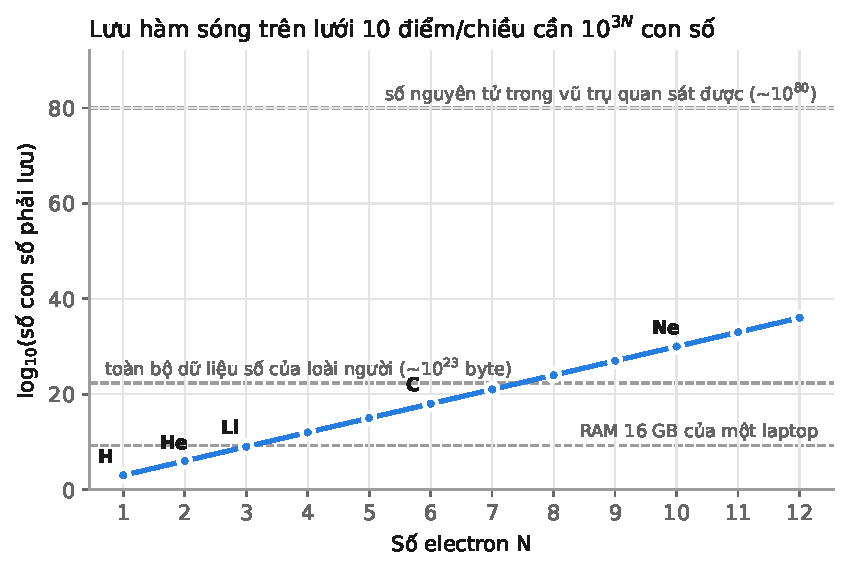
\includegraphics[width=0.86\textwidth]{01_buc_tuong_ham_mu.pdf}
\caption{Số con số cần lưu để ghi hàm sóng của $N$ electron trên lưới 10 điểm mỗi chiều: $10^{3N}$. Trục tung dùng thang log nên đường thẳng nghĩa là tăng theo hàm mũ. Ba vạch ngang là RAM laptop, toàn bộ dữ liệu số của loài người, và số nguyên tử trong vũ trụ. (Script \code{01\_nen\_tang.py})}
\label{fig:buctuong}
\end{figure}

Walter Kohn gọi hiện tượng này là \textbf{bức tường hàm mũ} \en{exponential wall} trong bài giảng nhận giải Nobel năm 1998 \cite{Kohn1999}. Lập luận của ông: để năng lượng chính xác cỡ 1\%, mỗi tọa độ cần khoảng $p = 3$ đến $10$ tham số, nên tổng số tham số là
\[
M = p^{3N}.
\]
Nếu máy tính tốt nhất xử lý được $\bar M\approx10^9$ tham số với $p=3$, thì số electron tối đa là $\bar N = \frac13\log_{10}\bar M/\log_{10} p\approx 6$. Kohn viết: \emph{``Let us optimistically take $\bar M\approx10^9$ and $p=3$. This gives the shocking result $\bar N=\frac13\cdot\frac{9}{0.48}=6$ (!)''}, và \emph{``the exponential in Eq.~(2.12) represents a `wall' severely limiting $\bar N$''}. Với 100 electron, $M\approx3^{300}\approx10^{143}$, một con số không có ý nghĩa thực tế nào.

Bức tường không chỉ xuất hiện khi dùng lưới. Chương~\ref{ch:sauhf} sẽ cho thấy cách viết hàm sóng bằng tổ hợp các ``cấu hình electron'' (Full CI) cũng gặp đúng bức tường này dưới dạng tổ hợp.

\section{Câu nói của Dirac}

Năm 1929, chỉ ba năm sau phương trình Schrödinger, Paul Dirac viết một câu đã trở thành ``tuyên ngôn'' của ngành hóa học tính toán \cite{Dirac1929}:

\begin{quote}
\itshape ``The underlying physical laws necessary for the mathematical theory of a large part of physics and the whole of chemistry are thus completely known, and the difficulty is only that the exact application of these laws leads to equations much too complicated to be soluble. It therefore becomes desirable that approximate practical methods of applying quantum mechanics should be developed\ldots''
\end{quote}
Tạm dịch: \emph{Các định luật vật lý nền tảng cho phần lớn vật lý và toàn bộ hóa học đã được biết đầy đủ. Cái khó chỉ là việc áp dụng chính xác các định luật này dẫn tới những phương trình quá phức tạp để giải được. Vì vậy cần phát triển các phương pháp gần đúng thực tế\ldots}

Toàn bộ phần còn lại của tài liệu là câu chuyện về các ``phương pháp gần đúng thực tế'' đó.

\begin{ghinho}
\begin{itemize}
\item Hamiltonian của nguyên tử $N$ electron gồm động năng, hút hạt nhân, và $N(N-1)/2$ số hạng đẩy nhau $1/r_{ij}$. Chính các số hạng đẩy nhau làm bài toán không tách biến được.
\item Bỏ lực đẩy, Li cho $-10.125\Ha$ (sai 35\%). Lực đẩy không phải ``hiệu chỉnh nhỏ''.
\item Hàm sóng $N$ electron sống trong không gian $3N$ chiều. Lưu nó một cách ngây thơ cần $\sim10^{3N}$ con số: bức tường hàm mũ.
\item ``Không có công thức'' khác ``không biết đáp án'': năng lượng Li đã biết tới 15 chữ số, $-7.478\,060\,323\,910\Ha$. Ta sẽ dùng con số này làm trọng tài cho mọi phương pháp.
\end{itemize}
\end{ghinho}
